\section{Systemdesign}

% TODO: Flytta rubrikerna till rätt filer.

\subsection{Språk}
Programmet som skall lösa optimeringsproblemmet skrivs i programmeringsspråket C. 

\subsection{Standarder}
Källkoden följer de standarder som är beskrivna i kvalitetsplanen.

\subsection{Systemskiss}
Programmet kommer i huvudsak köras via matlab, där kommer programmet anropas som en funktion med all indata i parametrarna. Indatan kommer sedan kompileras till en header fil som sedan skickas till mex solvern. QP-solvern kommer sedan lösa problemet utifrån kompilerade datan och sedan returnera resultatet till matlab. Programmet kommer även att kunna köras från vårt eget GUI, där man i GUI:t kan mata in sitt QP problem och de matriser man vill använda, generera en C problem fil som kan lösas av C solvern. Resultatet skickas sedan tillbaka och visas i GUI:t.

\begin{figure}[h]
	\begin{center}
		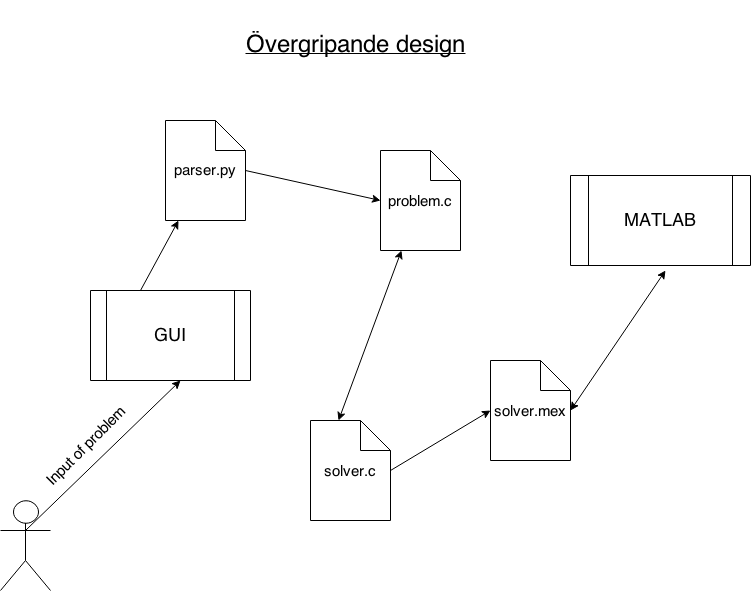
\includegraphics[scale=0.5]{bilder/overgripande.png}
	\end{center}
\end{figure}

\subsection{Enkel problembeskrivning}
Detta är en enkel beskrivning på vårt koncept om hur programmet ska fungera. Man har ett konvext kvadratiskt minimeringsproblem som man vill lösa. Problemet skickas till vårt program som med av oss utvalda effektiva algoritmer räknar ut den optimala lösningen \textit{z*}.

\begin{figure}[h]
	\begin{center}
		\includegraphics[scale=0.5]{bilder/generellt.png}
	\end{center}
\end{figure}

%% Graphic for TeX using PGF
% Title: C:\Users\sebfas\Pictures\Systemskiss.dia
% Creator: Dia v0.97.2
% CreationDate: Sun Feb 15 00:30:41 2015
% For: sebfas
% \usepackage{tikz}
% The following commands are not supported in PSTricks at present
% We define them conditionally, so when they are implemented,
% this pgf file will use them.
\ifx\du\undefined
  \newlength{\du}
\fi
\setlength{\du}{15\unitlength}
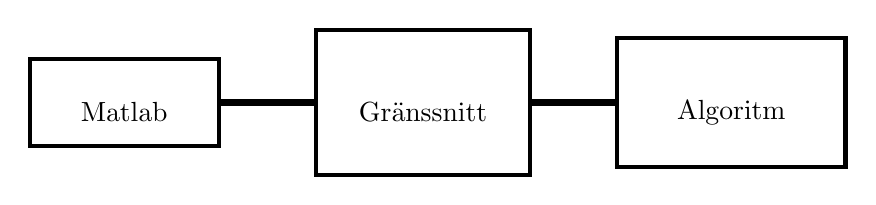
\begin{tikzpicture}
\pgftransformxscale{1.000000}
\pgftransformyscale{-1.000000}
\definecolor{dialinecolor}{rgb}{0.000000, 0.000000, 0.000000}
\pgfsetstrokecolor{dialinecolor}
\definecolor{dialinecolor}{rgb}{1.000000, 1.000000, 1.000000}
\pgfsetfillcolor{dialinecolor}
\definecolor{dialinecolor}{rgb}{1.000000, 1.000000, 1.000000}
\pgfsetfillcolor{dialinecolor}
\fill (1.400000\du,1.700000\du)--(1.400000\du,3.800000\du)--(5.950000\du,3.800000\du)--(5.950000\du,1.700000\du)--cycle;
\pgfsetlinewidth{0.100000\du}
\pgfsetdash{}{0pt}
\pgfsetdash{}{0pt}
\pgfsetmiterjoin
\definecolor{dialinecolor}{rgb}{0.000000, 0.000000, 0.000000}
\pgfsetstrokecolor{dialinecolor}
\draw (1.400000\du,1.700000\du)--(1.400000\du,3.800000\du)--(5.950000\du,3.800000\du)--(5.950000\du,1.700000\du)--cycle;
% setfont left to latex
\definecolor{dialinecolor}{rgb}{0.000000, 0.000000, 0.000000}
\pgfsetstrokecolor{dialinecolor}
\node at (3.675000\du,2.990000\du){Matlab};
\definecolor{dialinecolor}{rgb}{1.000000, 1.000000, 1.000000}
\pgfsetfillcolor{dialinecolor}
\fill (8.300000\du,1.000000\du)--(8.300000\du,4.500000\du)--(13.450000\du,4.500000\du)--(13.450000\du,1.000000\du)--cycle;
\pgfsetlinewidth{0.100000\du}
\pgfsetdash{}{0pt}
\pgfsetdash{}{0pt}
\pgfsetmiterjoin
\definecolor{dialinecolor}{rgb}{0.000000, 0.000000, 0.000000}
\pgfsetstrokecolor{dialinecolor}
\draw (8.300000\du,1.000000\du)--(8.300000\du,4.500000\du)--(13.450000\du,4.500000\du)--(13.450000\du,1.000000\du)--cycle;
% setfont left to latex
\definecolor{dialinecolor}{rgb}{0.000000, 0.000000, 0.000000}
\pgfsetstrokecolor{dialinecolor}
\node at (10.875000\du,2.990000\du){Gränssnitt};
\definecolor{dialinecolor}{rgb}{1.000000, 1.000000, 1.000000}
\pgfsetfillcolor{dialinecolor}
\fill (15.550000\du,1.200000\du)--(15.550000\du,4.300000\du)--(21.050000\du,4.300000\du)--(21.050000\du,1.200000\du)--cycle;
\pgfsetlinewidth{0.100000\du}
\pgfsetdash{}{0pt}
\pgfsetdash{}{0pt}
\pgfsetmiterjoin
\definecolor{dialinecolor}{rgb}{0.000000, 0.000000, 0.000000}
\pgfsetstrokecolor{dialinecolor}
\draw (15.550000\du,1.200000\du)--(15.550000\du,4.300000\du)--(21.050000\du,4.300000\du)--(21.050000\du,1.200000\du)--cycle;
% setfont left to latex
\definecolor{dialinecolor}{rgb}{0.000000, 0.000000, 0.000000}
\pgfsetstrokecolor{dialinecolor}
\node at (18.300000\du,2.990000\du){Algoritm};
\pgfsetlinewidth{0.150000\du}
\pgfsetdash{}{0pt}
\pgfsetdash{}{0pt}
\pgfsetbuttcap
{
\definecolor{dialinecolor}{rgb}{0.000000, 0.000000, 0.000000}
\pgfsetfillcolor{dialinecolor}
% was here!!!
\definecolor{dialinecolor}{rgb}{0.000000, 0.000000, 0.000000}
\pgfsetstrokecolor{dialinecolor}
\draw (5.950000\du,2.750000\du)--(8.300000\du,2.750000\du);
}
\pgfsetlinewidth{0.150000\du}
\pgfsetdash{}{0pt}
\pgfsetdash{}{0pt}
\pgfsetbuttcap
{
\definecolor{dialinecolor}{rgb}{0.000000, 0.000000, 0.000000}
\pgfsetfillcolor{dialinecolor}
% was here!!!
\definecolor{dialinecolor}{rgb}{0.000000, 0.000000, 0.000000}
\pgfsetstrokecolor{dialinecolor}
\draw (13.450000\du,2.750000\du)--(15.550000\du,2.750000\du);
}
\end{tikzpicture}


\subsection{Syfte}
Syftet med arkitekturen är att skapa en översikt av hela systemet för att man på ett enkelt sätt ska få en överblick av hur alla moduler hänger ihop och hur de fungerar. Den är även ett underlag för att kunna skapa den slutgiltliga tekniska dokumentationen.

\subsection{Prestanda}
Det är av yttersta vikt att programmet löser QP-problemet väldigt snabbt, i samma skala som Gurobi. Detta är dels för att flygplanet ska hinna utföra prediktionsregleringen i tid.

\subsection{Stabilitet}
Eftersom tanken med programmet är att lösa kvadratiska problem för preditionsreglering åt stridsflygplan så är det väldigt viktigt att det inte blir några fel i programmet, detta löses med validering av indata.

\subsection{GUI}
GUI:t används för att mata in de matriser som behövs för att lösa problemet. GUI:t kommer att anropa \textit{parser.py} med de inmatade matriserna.

\subsection{parser.py}
Gör om den indatan som kommer från GUI:t till filen \textit{problem.c} innehållande alla matriser med specificerade dimensioner som solvern kommer behöva för att lösa problemet.

\subsection{problem.c}
Är den genererade datafilen från \textit{parser.py} som innehåller alla de matriser som solvern behöver för att lösa problemet skriven med samma datatyper som solvern kommer att behöva använda. Dessa matriser är bivillkorsmatriserna A, B, F och G.  

\subsection{solver.c}
Innehåller metoderna för att lösa QP-problemet, där algoritmen är uppdelad i flera olika steg.

\subsection{solver.mex}
Kommer att fungera som \textit{solver.c} fast den kommer att kunna anropas via Matlab istället för vårt GUI. Programmet kommer att köras genom att anropa en funktion i Matlab med matriserna i parametrarna som indata.

%\subsection{Arkitekturens delar}
%Arkitekturen är uppdelad i tre större delar där GUI:t och parsern är en del
%Lösningsalgoritmen solvern är en del ... active-set-metoden
%Integrationen mot matlab är en del ... funktioner...

\subsection{Matrisbibliotek}
Arkitekturen innehåller även ett eget matrisbibliotek, innehållande alla nödvändiga matrisoperationer för lösaren.

